% !TEX encoding = UTF-8
% !TEX TS-program = pdflatex
% !TEX root = ../../tesi.tex

\section{Analisi dei requisiti}
Ho iniziato la fase di analisi dei requisiti dalla quarta settimana di lavoro, cioè quando, come pianificato, avrei dovuto iniziare ad implementare gli \textit{smart contract} per la gestione di NFT seguendo gli standard ERC su \textit{blockchain} Ethereum. Inizialmente è avvenuto un processo di \textit{brainstorming} con gli altri componenti del gruppo e i vari \textit{tutor} di ognuno di noi per definire al meglio le funzionalità della piattaforma. In seguito ho isolato e ridotto le funzionalità ed i requisiti che avrebbe dovuto la mia libreria e lo \textit{smart contract} che avrei dovuto implementare. Per quanto riguarda i casi d'uso, vengono utilizzati i diagrammi dei casi d'uso per facilitarne la Presentazione concettuale, mentre per i requisiti sono state utilizzate delle tabelle di tracciamento. 

\subsection{Casi d'uso}
I casi d'uso sono una tecnica utilizzata nel processo di analisi dei requisiti per effettuare in maniera esaustiva e non ambigua, la raccolta dei requisiti al fine di produrre \textit{software} di qualità. \\

\noindent La classificazione dei casi d'uso ha seguito la seguente convenzione:
\begin{center}
  UC[NumeroCasoBase](.[NumeroSottoCaso])*
\end{center}
dove:
\begin{itemize}
  \item \textbf{NumeroCasoBase}: è costituito da un numero progressivo che indica il caso d'uso generico;
  \item \textbf{NumeroSottoCaso}: è costituito da un numero progressivo opzionale che indica il sotto-caso d'uso del caso
  d'uso generico.
\end{itemize}

\subsubsection{Attori primari}
Un attore primario è colui che interagisce con il sistema per un determinato scopo.
Gli attori primari identificati sono i seguenti:

\begin{figure}[h!]
  \centering
  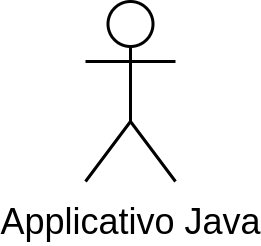
\includegraphics{capitolo3/casi-uso/attori-primari.png}
  \caption{Attori primari}
\end{figure}

\begin{itemize}
  \item \textbf{Applicativo Java}: rappresenta qualsiasi applicazione sviluppata in Java che interagisce con la libreria. In questo caso, consiste nel \textit{back-end} sviluppato utilizzando il \textit{framework} Spring.
\end{itemize}

\subsubsection{Attori secondari}
Un attore secondario è un'entità estranea al sistema che supporta gli attori primari nelle loro attività.

\begin{figure}[h!]
  \centering
  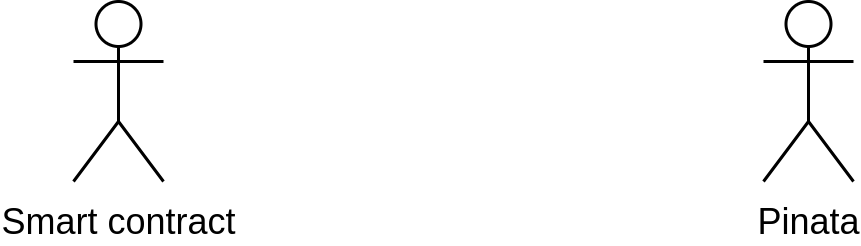
\includegraphics{capitolo3/casi-uso/attori-secondari.png}
  \caption{Attori secondari}
\end{figure}

\begin{itemize}
  \item \textbf{\textit{Smart contract}}: rappresenta lo \textit{smart contract} caricato in \textit{blockchain} con il quale comunicare;
  \item \textbf{Pinata}: rappresenta il servizio che permette di interagire con la rete IPFS.
\end{itemize}

\UC{Caricamento di un opera in blockchain}
Qualsiasi applicativo Java può caricare un opera in blockchain.

\begin{itemize}
  \item \UCPrimaryActors{applicativo Java};
  \item \UCSecondaryActors{smart contract, Pinata};
  \item \UCPre{l'applicativo Java vuole creare un NFT da un opera non ancora esistente};
  \item \UCPost{il NFT è stato creato e l'opera è stata caricata nella rete IPFS};
  \item \UCMain{}
  \begin{itemize}
    \item L'applicativo Java vuole creare un NFT a partire da un opera, dalla quale non è stato creato alcun NFT;
    \item L'opera viene caricata sulla rete IPFS tramite il servizio Pinata;
    \item Viene contattato lo \textit{smart contract} e creato il NFT.
  \end{itemize}
  \item \UCExt{}
  \begin{enumerate}[label=\lett]
    \item L'applicativo Java vuole comunicare con lo \textit{smart contract} attraverso un \textit{wallet}, il quale non è il proprietario dello \textit{smart contract}:
    \begin{itemize}
      \item (UC\ref{UC:extension.operation-not-allowed}) - Visualizzazione messaggio di operazione non consentita;
      \item Viene impedita la creazione del NFT.
    \end{itemize}

    \item L'applicativo Java vuole caricare un'opera dalla quale è già stato estratto il NFT:
    \begin{itemize}
      \item (UC\ref{UC:extension.opera-exists-yet}) - Visualizzazione messaggio di opera già esistente;
      \item Viene impedita la creazione del NFT.
    \end{itemize}
  \end{enumerate}
\end{itemize}


\UC{Vendita di un opera}
L'applicativo Java può trasferire la proprietà di un'opera dal proprietario all'acquirente.

\begin{itemize}
  \item 
\end{itemize}

\UC{Ottenimento di un opera a partire dal suo id}

\UC{Ottenimento di un opera a partire dal suo hash}

\UC{Ottenimento della storia delle transazioni di un opera}

\UC{Visualizzazione messaggio di operazione con consentita}
\label{UC:extension.operation-not-allowed}

\UC{Visualizzazione messaggio di opera già esistente}
\label{UC:extension.opera-exists-yet}


% \paragraph{UC1 - Caricamento di un opera in blockchain}

% \paragraph{UC2 - Vendita di un opera}

% \paragraph{UC3 - Ottenimento di un opera a partire dal suo id}

% \paragraph{UC4 - Ottenimento di un opera a partire dal suo hash}

\subsection{Requisiti funzionali}
Tabella dei requisiti funzionali, con relativa spiegazione e fonte.

\subsection{Requisiti di qualità}
Tabella dei requisiti di qualità, con relativa spiegazione e fonte.

\subsection{Requisiti di vincolo}
Tabella dei requisiti di vincolo, con relativa spiegazione e fonte.